
\documentclass{beamer}
\usetheme{Madrid}
\usepackage{url}
\usepackage{subfig}
\usepackage{multimedia}

\title{The spreading of (fake) news in social networks}
\author{FATTJ}
\institute{ETH Zurich}
\date{\today}


\begin{document}
\titlepage

\begin{frame}
\frametitle{Outline}
\tableofcontents
\end{frame}

\begin{frame}{Introduction}
\begin{figure}

\includegraphics[scale=0.4]{images/TrumpFakeNews.png}
\caption{Trump Tweet}
\end{figure}
\end{frame}


\section{Introduction}

\begin{frame}{Goal}
The goal of our project has been to construct a model and simulation code to better understand the spread of (fake) news on social media.
\end{frame}

\begin{frame}{Goal}
Give some insight into the following questions:
\begin{itemize}
\item<1-> How does network structure impact the spreading of a news?
\item<2-> What impact does the choice of initial spreaders have on the spreading of
competing news?
\item<3-> How can our understanding of the two previous questions be used to curb
the spreading of false news?
\end{itemize}
\end{frame}


\section{The Model}
% (2) The Model
\begin{frame}
\frametitle{Model Description}

\begin{center}
\begin{figure}
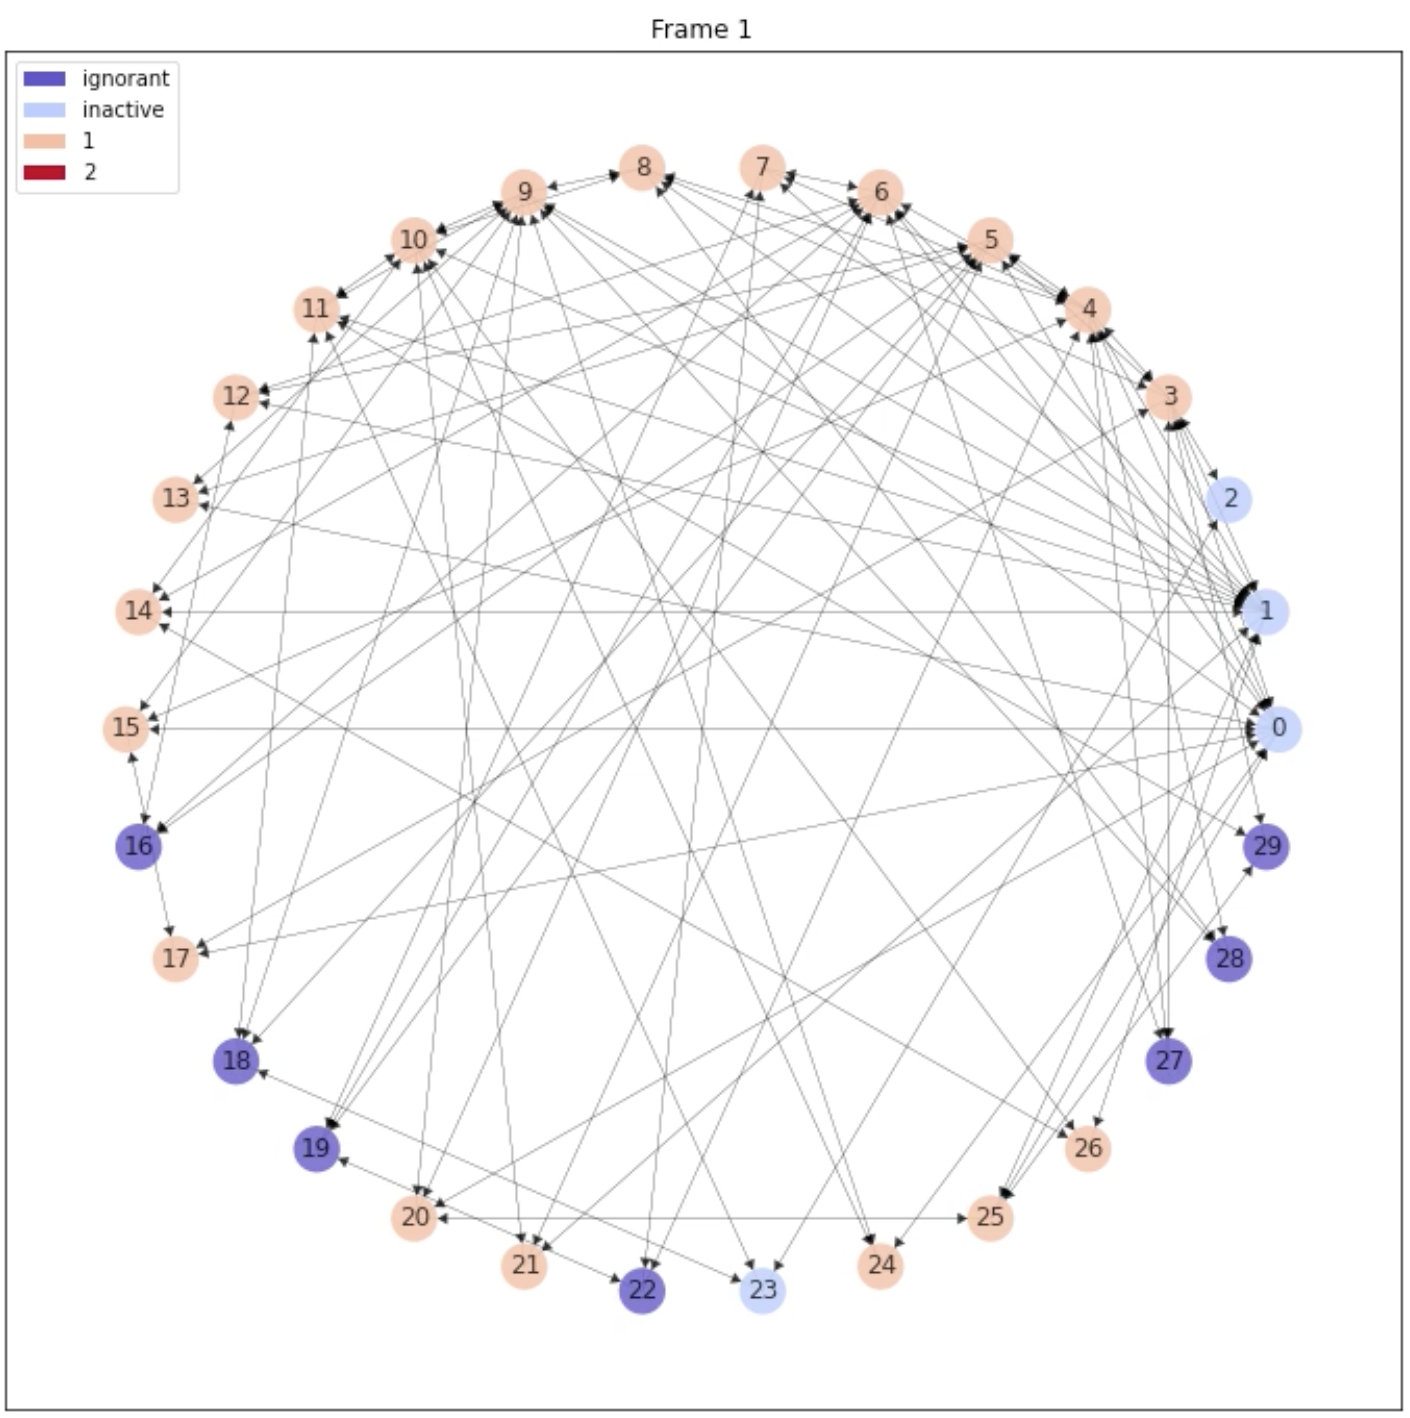
\includegraphics[scale=0.2]{images/frame_example.png}
\end{figure}
\end{center}

\begin{itemize}
\item<1-> Directed graph $G = (V,E)$
\item<2-> Node state: Ignorant, Inactive and Active
\item<3-> Receivers $R(v)$ and providers $P(v)$
\item<4-> Normalized weighted influence $\sum_{w \in P(v)} r_{v,w} = 1$
\end{itemize}

\end{frame}


\begin{frame}
\frametitle{Model Description}

\begin{center}
\begin{figure}
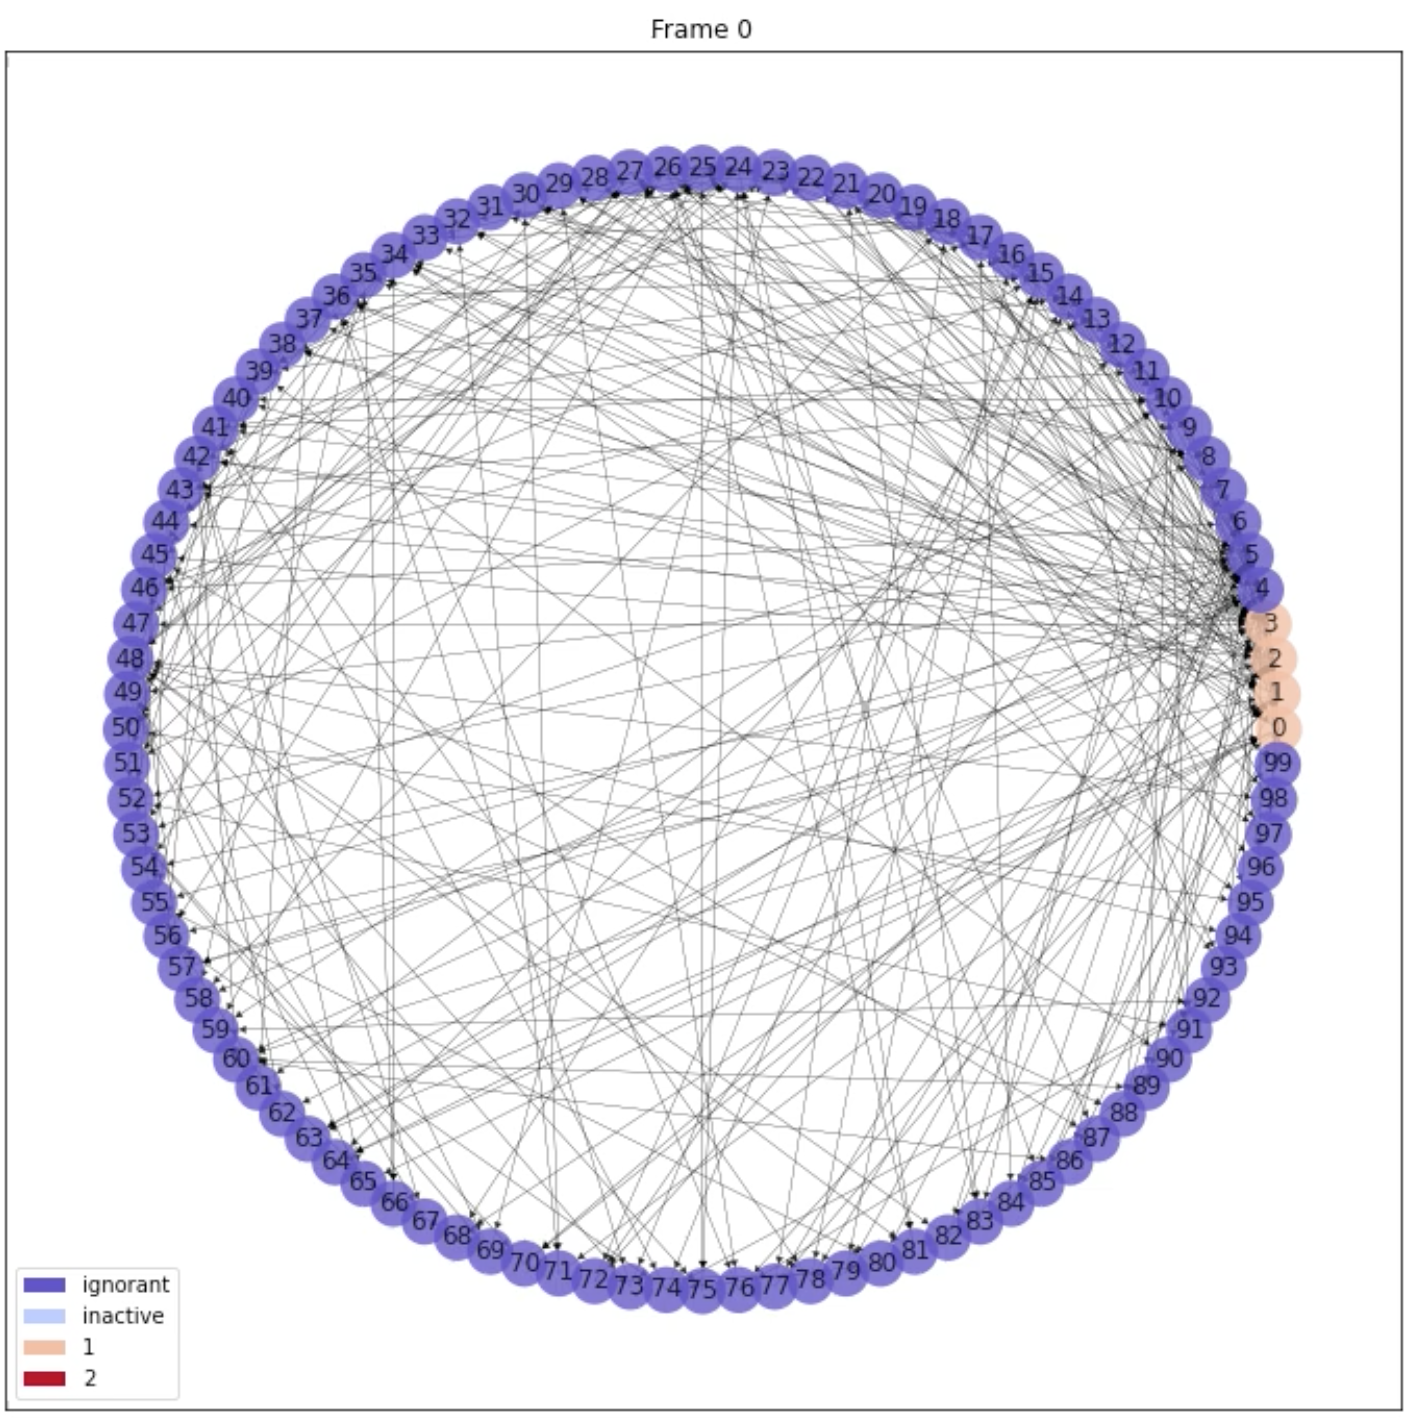
\includegraphics[scale=0.2]{images/frame0.png}
\end{figure}
\end{center}

\begin{itemize}
\item<1-> Initiators $A_0$
\item<2-> News with a given sensation $\rho(t)$
\end{itemize}

\end{frame}


\begin{frame}
\frametitle{Model Description}

\begin{center}
\begin{figure}
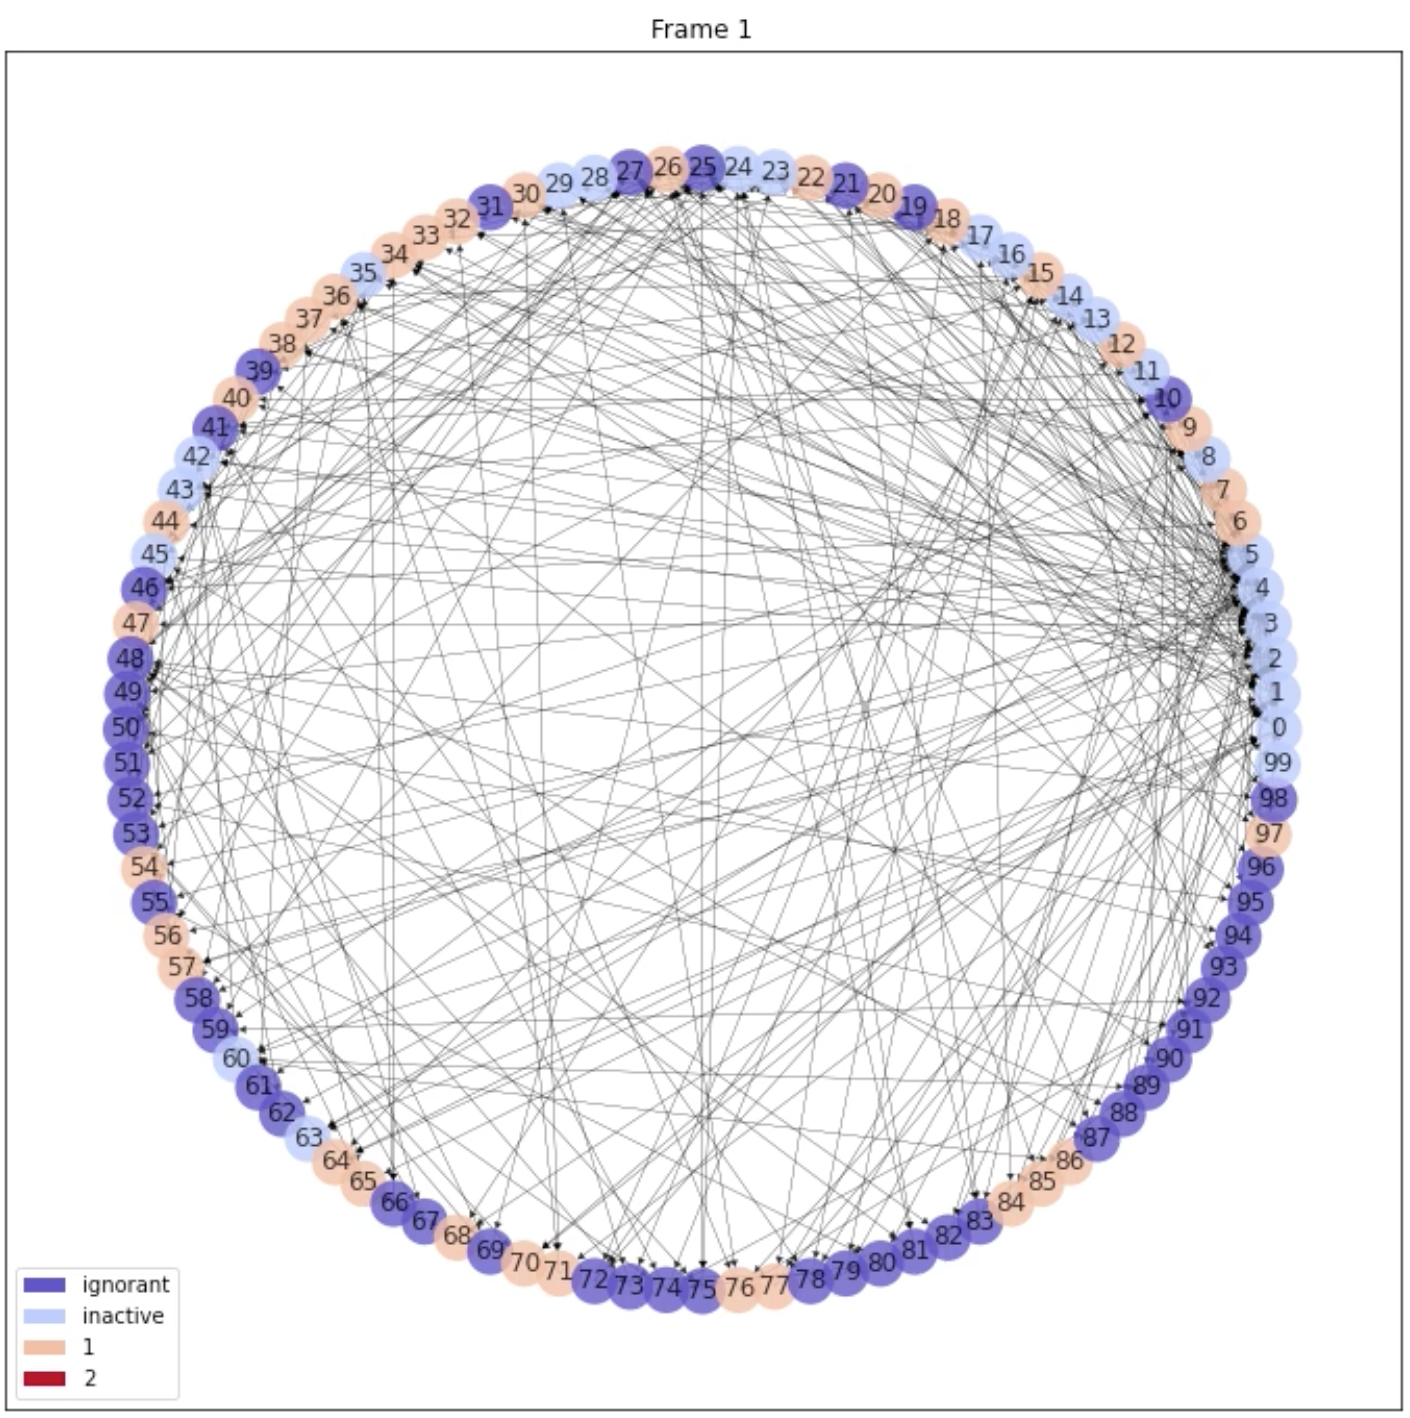
\includegraphics[scale=0.2]{images/frame1.png}
\end{figure}
\end{center}

\begin{itemize}
\item<1-> $t > 0$
\item<2-> Excitement $E_v\Big((r_{v,w})_{w \in P(v)}, \alpha_v \Big)$
\item<3-> Sharing the news if $E_v \geq  \phi_v \cdot c$
\end{itemize}

\end{frame}


\begin{frame}
\frametitle{Model Description}

\begin{center}
\begin{figure}
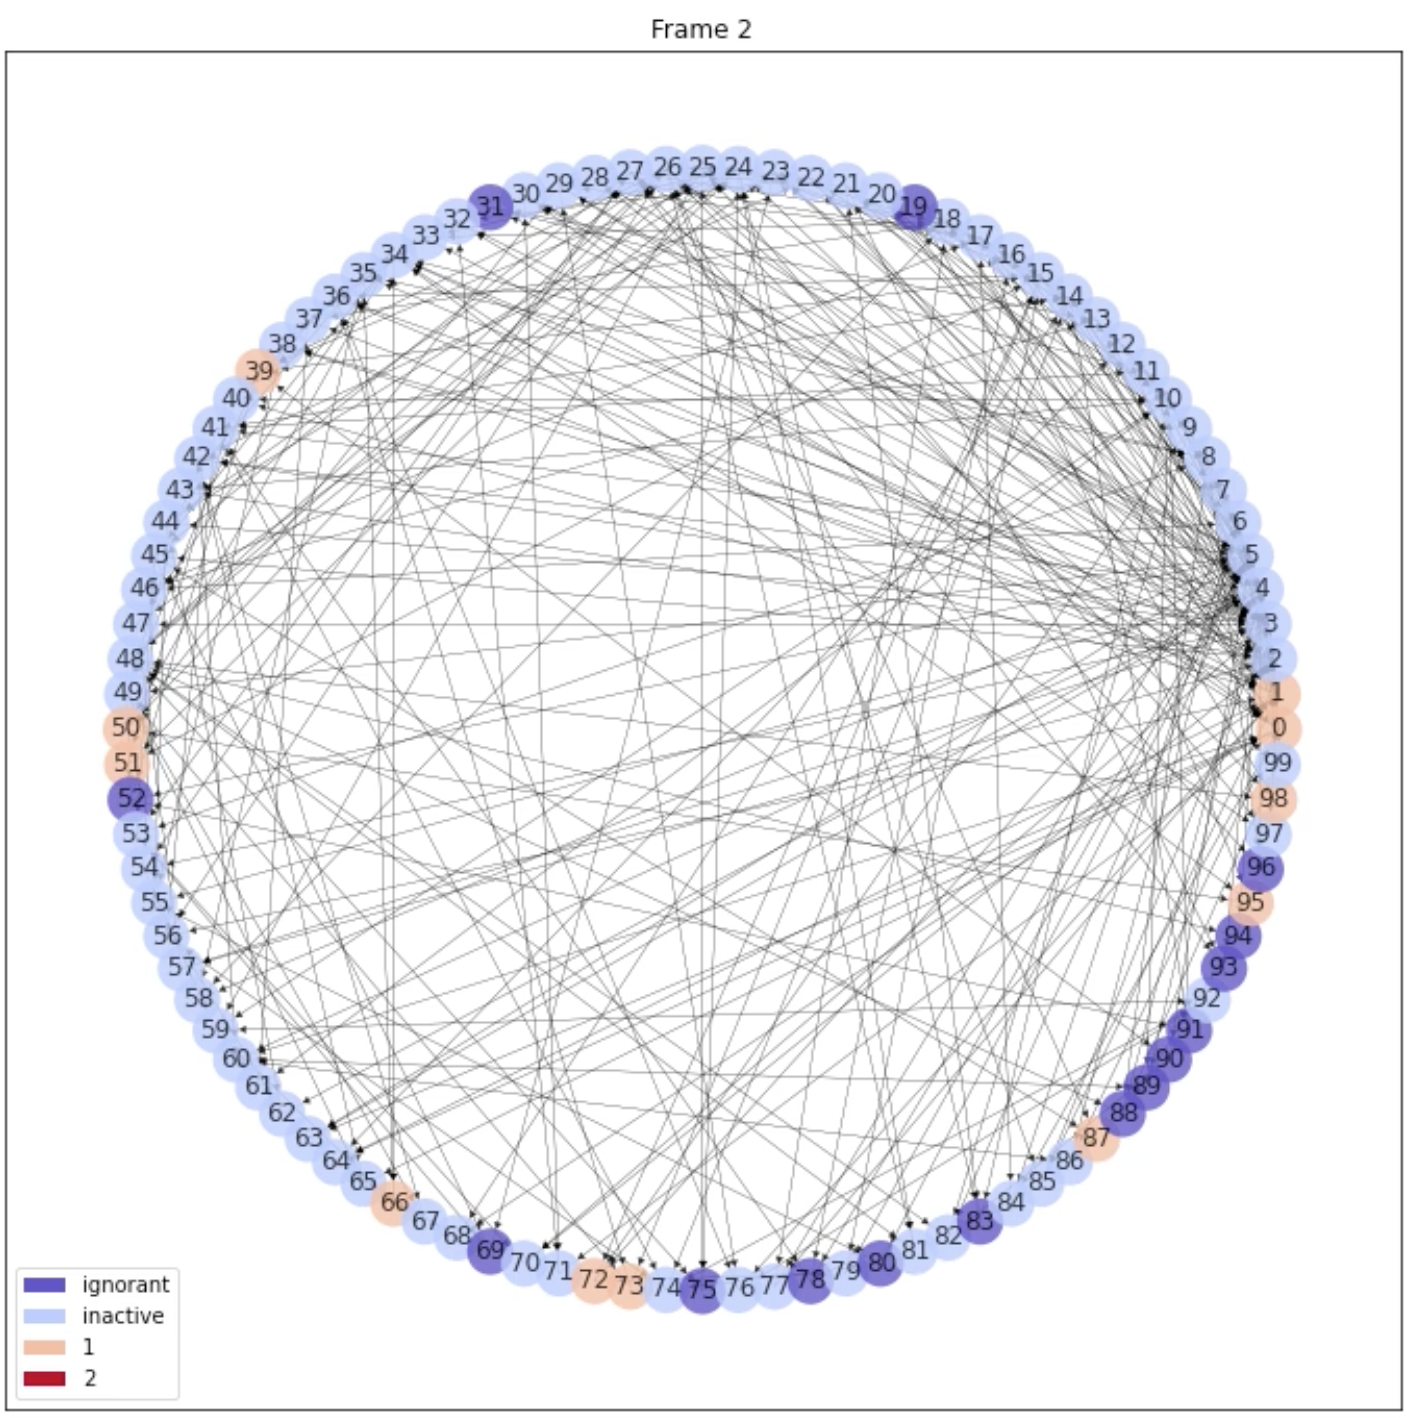
\includegraphics[scale=0.2]{images/frame2.png}
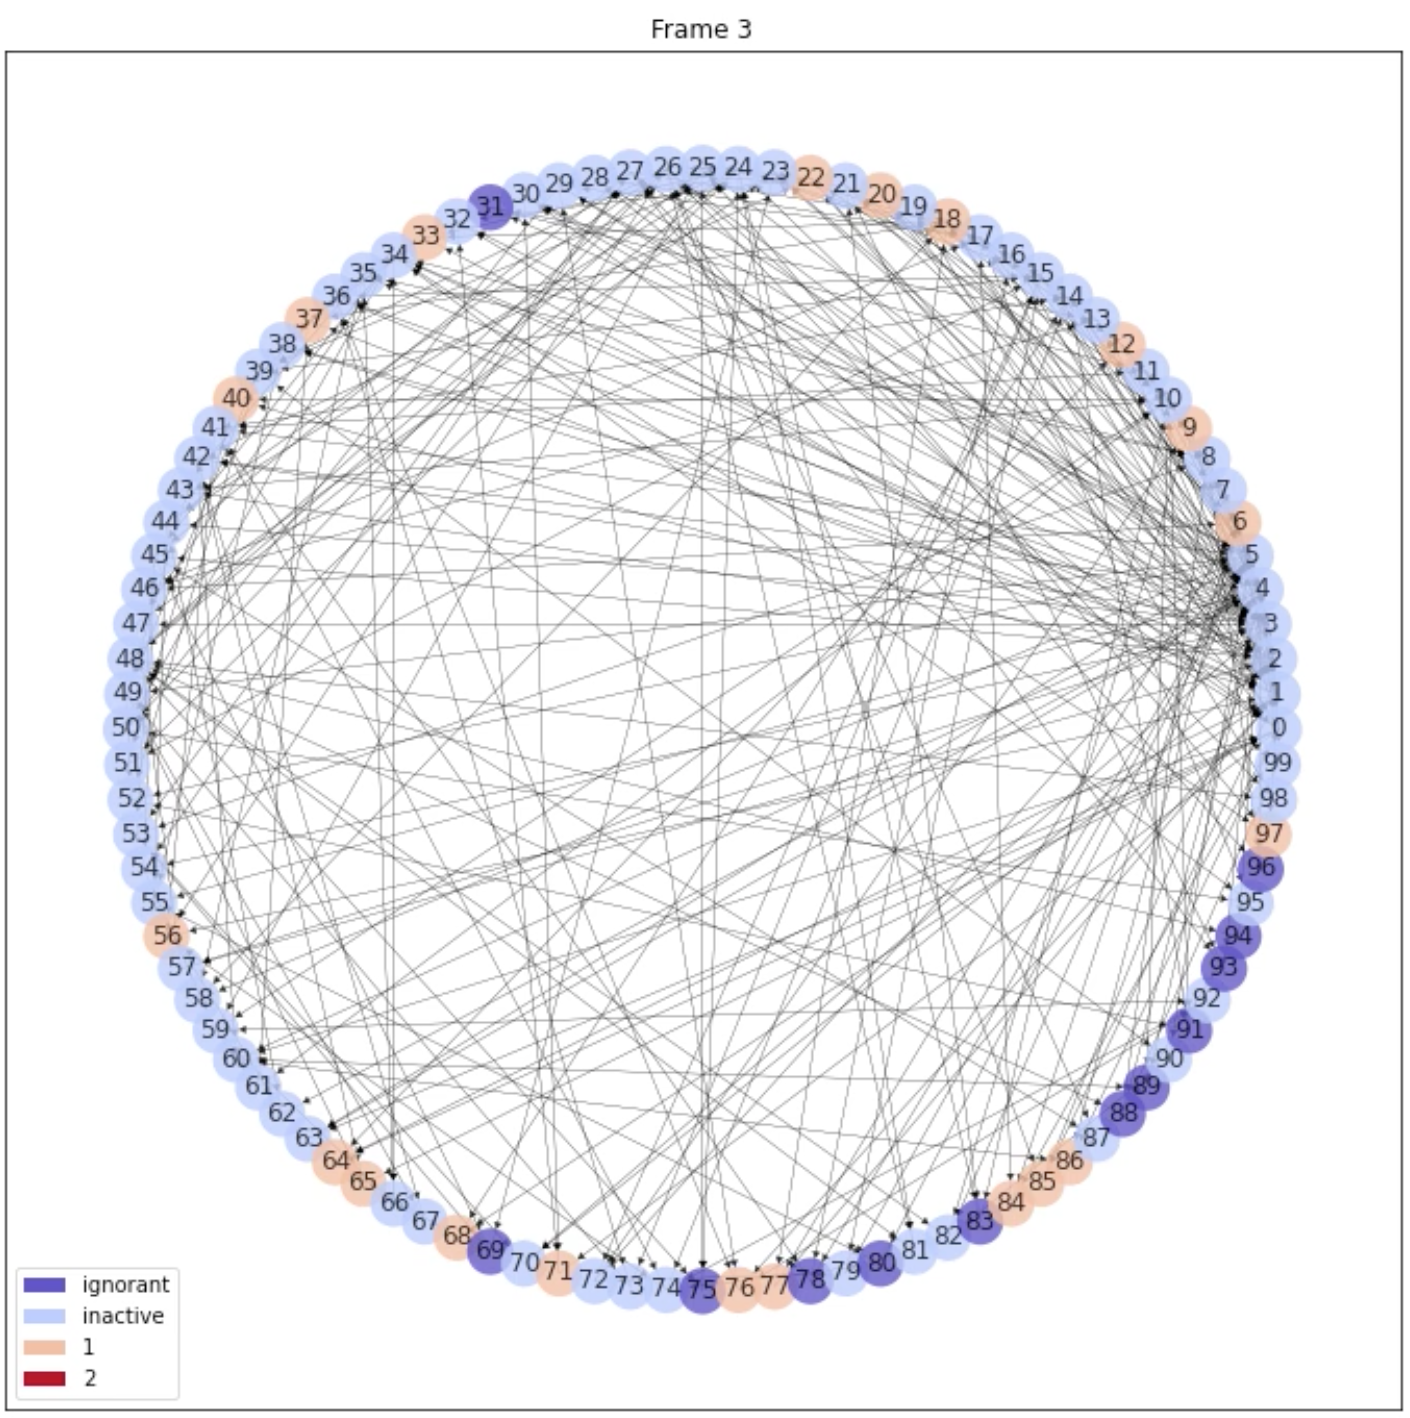
\includegraphics[scale=0.2]{images/frame3.png}
\end{figure}
\end{center}

\end{frame}


\begin{frame}
\frametitle{Model Description}

\begin{center}
\begin{figure}
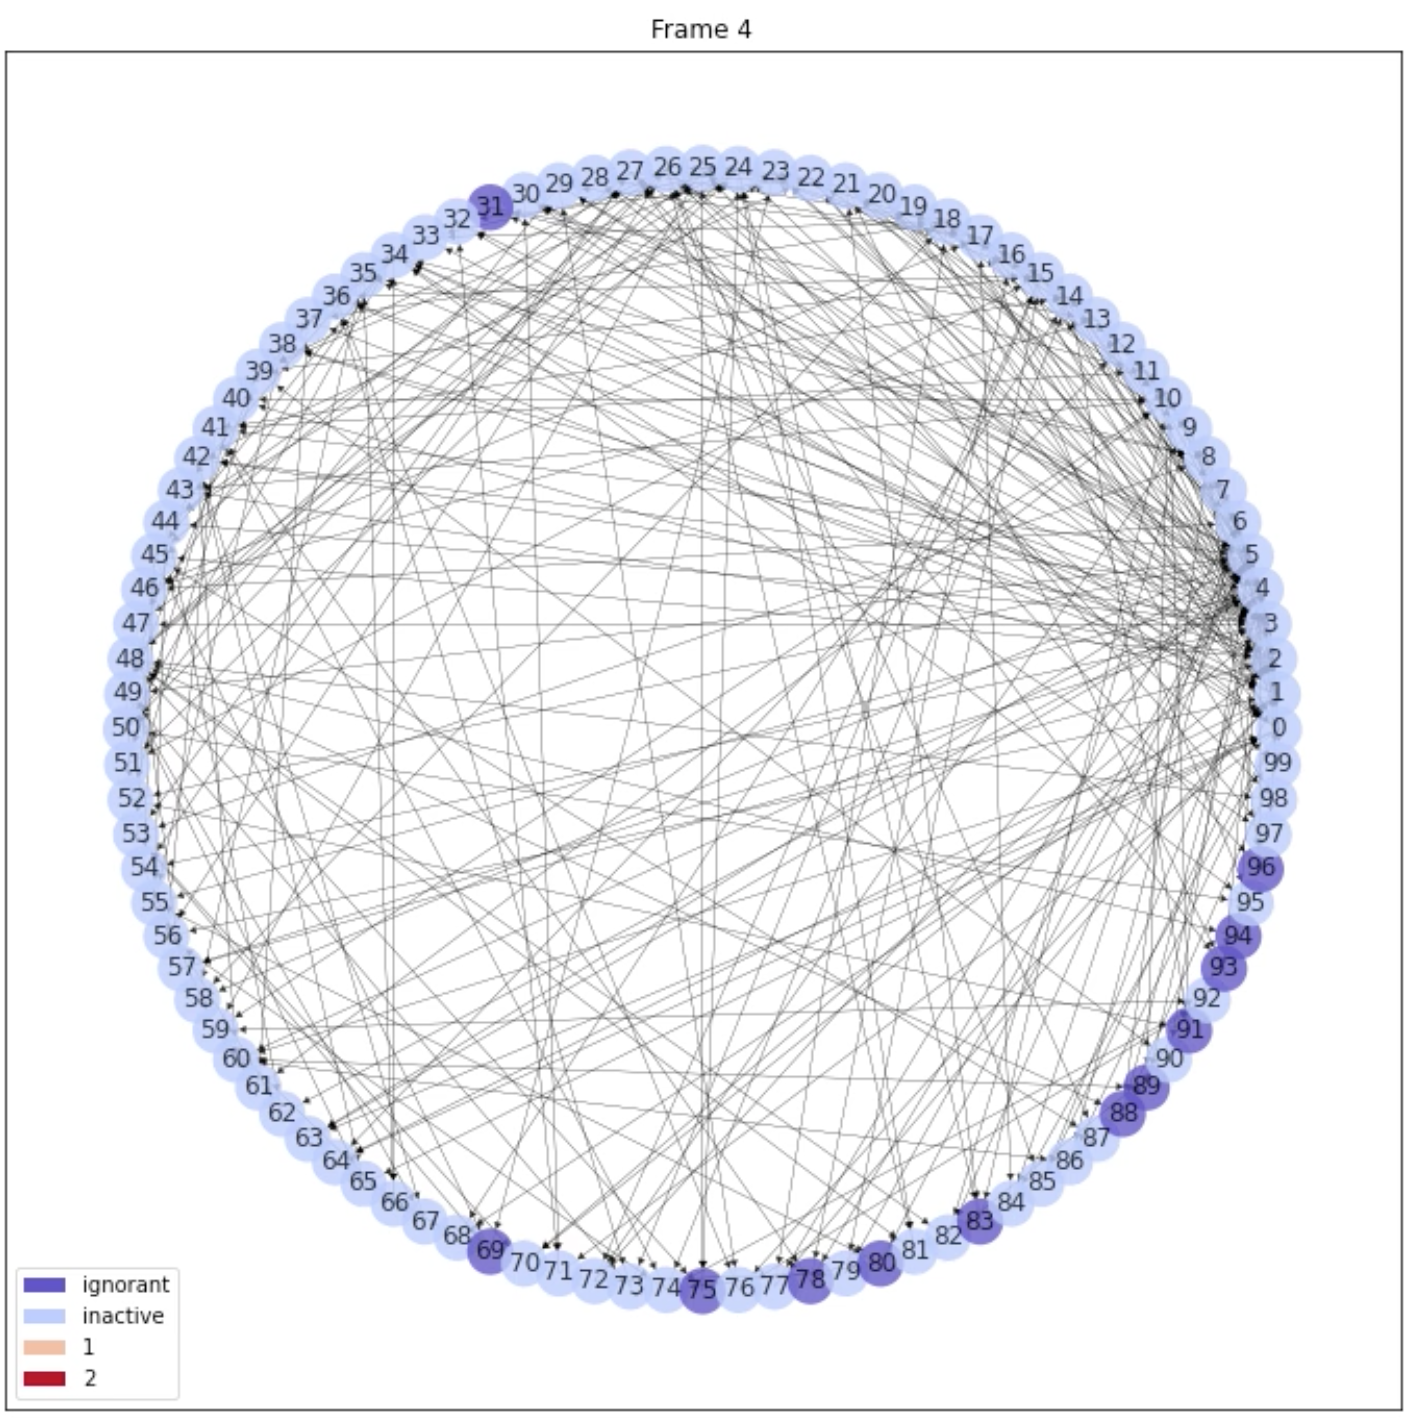
\includegraphics[scale=0.2]{images/frame4.png}
\end{figure}
\end{center}

\begin{itemize}
\item<1-> Until a stable situation is reached
\end{itemize}

\end{frame}



\section{Model evaluation}

\begin{frame}{Model evaluation}
    \begin{itemize}
        \item Get intuition for model parameter
        \item Cascade size: $C = \text{\#active agents} / \text{\#total agents}$
        \item Experiments with:
        \begin{itemize}
            \item Random parameters
            \item Power-law graph
        \end{itemize}
        \vspace{1cm}
        \item Expectations: Phase transitions
    \end{itemize}
\end{frame}

\begin{frame}{Model evaluation - Agent}
    \begin{itemize}
        \item Considered parameters:
        \begin{itemize}
            \item Threshold
            \item Independence
        \end{itemize}
        \item 1000 agents
        \item 50 samples
        \item 15 initial agents
    \end{itemize}
\end{frame}

\begin{frame}{Model evaluation - Agent}
    \begin{columns}
        \begin{column}{0.5\textwidth}
            \centering
            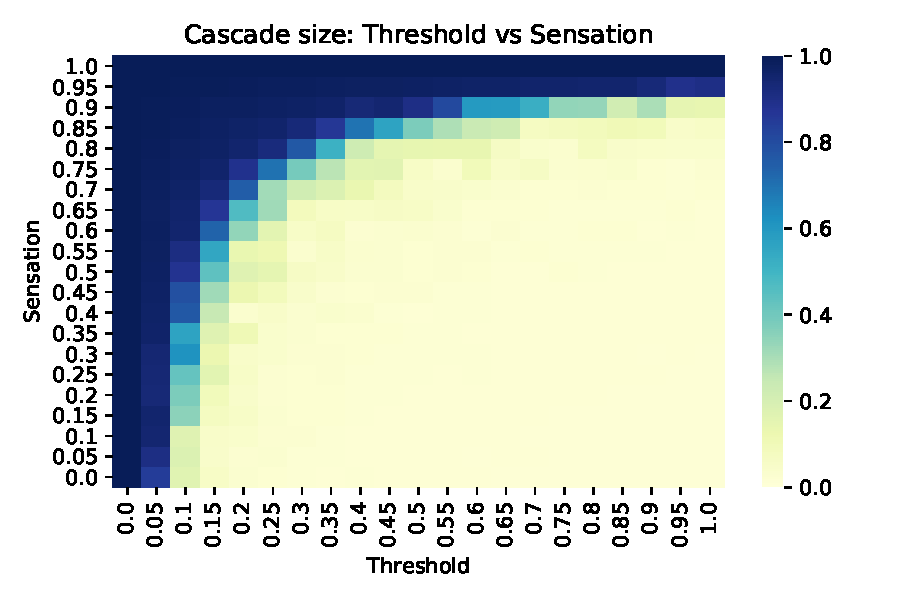
\includegraphics[width=0.95\textwidth]{images/threshold_sensation.pdf}
        \end{column}
        \begin{column}{0.5\textwidth}
            \centering
            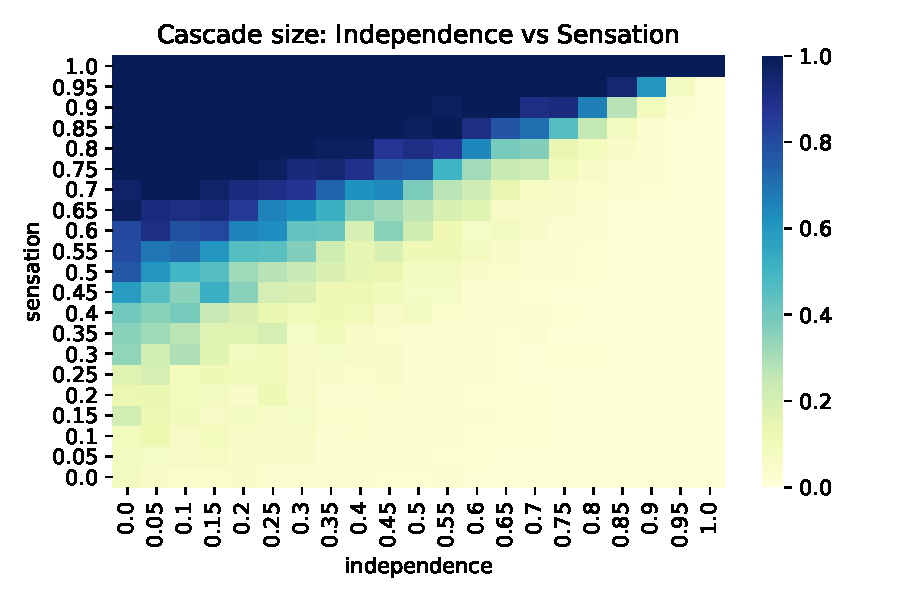
\includegraphics[width=0.95\textwidth]{images/independence_sensation.pdf}
        \end{column}
    \end{columns}
\end{frame}

\begin{frame}{Model evaluation - News}
    \begin{columns}
        \begin{column}{0.5\textwidth}
            \begin{itemize}
                \item Considered parameters:
                    \begin{itemize}
                        \item Decay parameter
                        \item Number of initial agents
                    \end{itemize}
                \item 1000 agents
                \item 50 samples
            \end{itemize}
        \end{column}
        \begin{column}{0.5\textwidth}
            \centering
            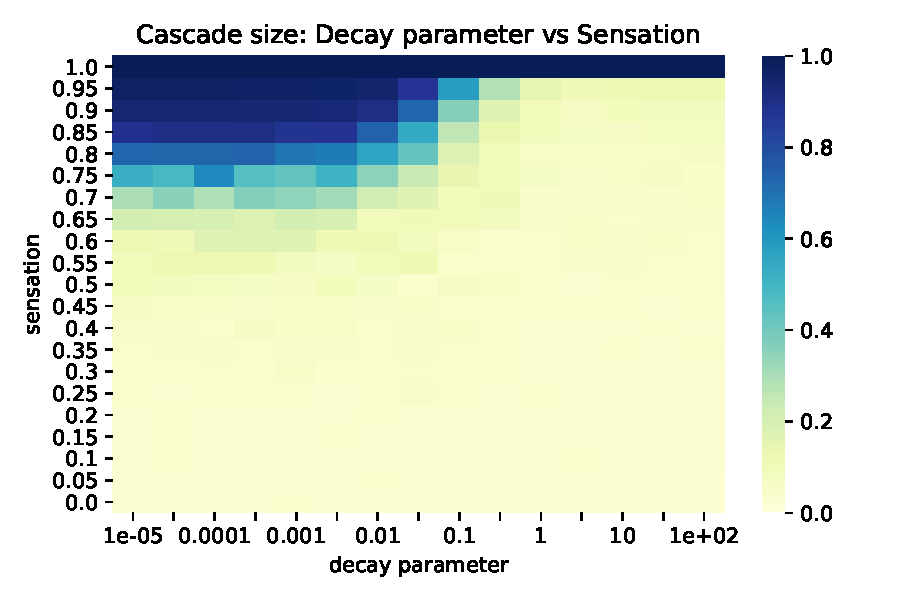
\includegraphics[width=0.95\textwidth]{images/decay_sensation.pdf}
        \end{column}
    \end{columns}
\end{frame}

\begin{frame}{Model evaluation - News}
    \begin{columns}
        \begin{column}{0.5\textwidth}
            \centering
            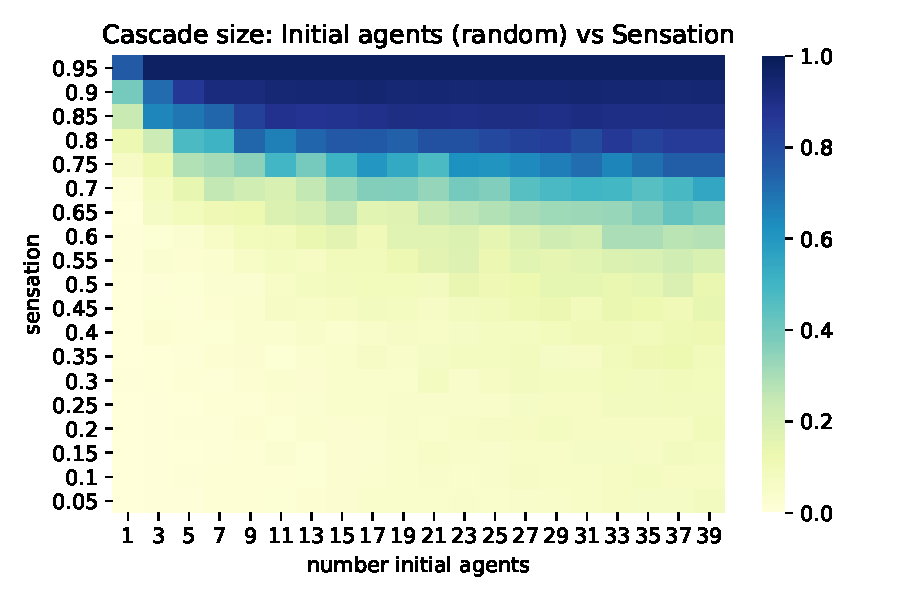
\includegraphics[width=0.95\textwidth]{images/initial_sensation_random.pdf}
        \end{column}
        \begin{column}{0.5\textwidth}
            \centering
            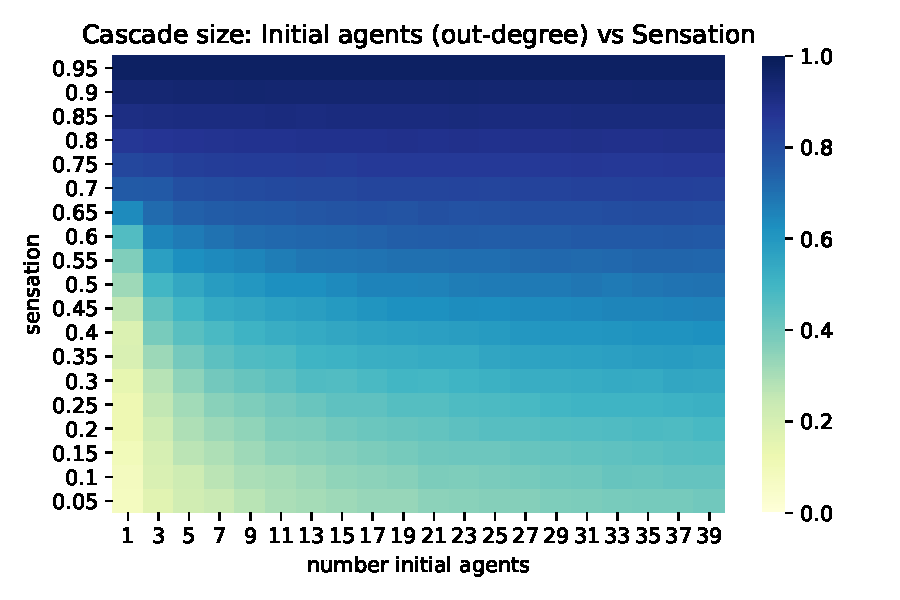
\includegraphics[width=0.95\textwidth]{images/initial_sensation_out_degree.pdf}
        \end{column}
    \end{columns}
\end{frame}

\section{Network Structure}


\begin{frame}
\frametitle{Network Structure: Construction of graph G(k, z)}
\begin{itemize}
\item Start with a connected graph in a circle, select one node as information provider
\item For every i = 1, ..., k: If i != 1: change information provider with probability z. Add edge with information provider and random information receiver.
\end{itemize}
\end{frame}

\begin{frame}
\frametitle{Network Structure: Some examples}
\begin{columns}
    \begin{column}{.4\textwidth}
    \centering
    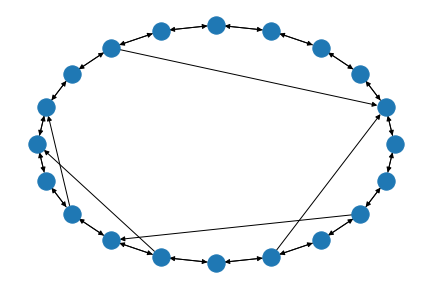
\includegraphics[width=.9\linewidth]{images/example2.png}
    \end{column}
    \begin{column}{.4\textwidth}
    \centering
    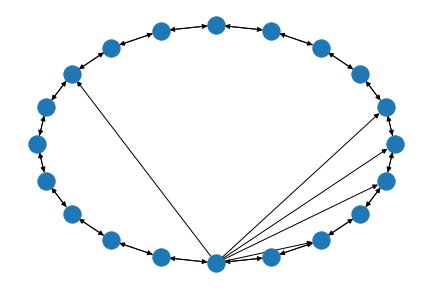
\includegraphics[width=.9\linewidth]{images/example8.png}
    \end{column}
\end{columns}
\begin{itemize}
    \item 20 nodes, 5 additional edges, c = 0.2 and c = 0.8
\end{itemize}
\end{frame}

\begin{frame}
\frametitle{Network Structure: Results}
\begin{columns}
    \begin{column}{.5\textwidth}
    \centering
    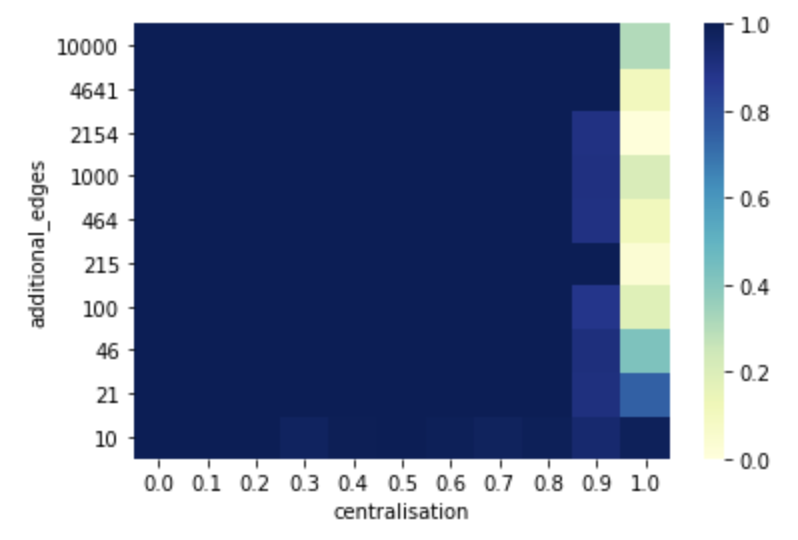
\includegraphics[width=.9\linewidth]{images/heatmap_graph_structure_09}
    \end{column}
    
    \begin{column}{.5\textwidth}
    \centering
    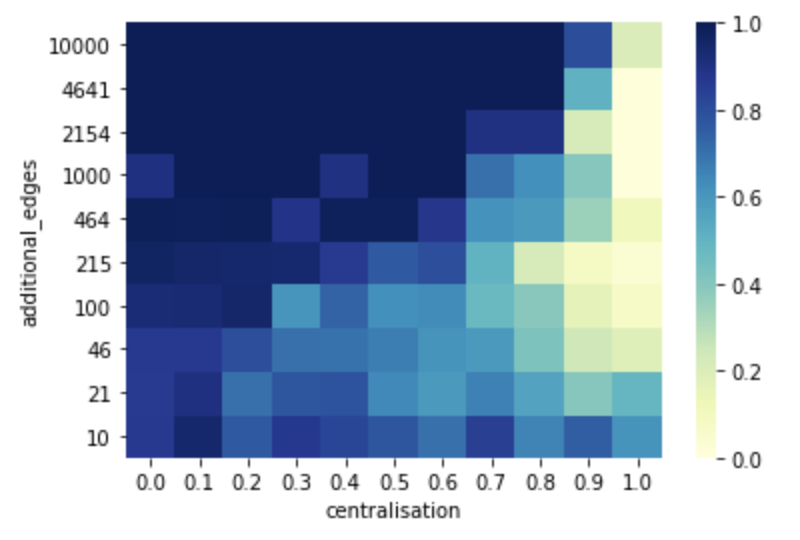
\includegraphics[width=.9\linewidth]{images/heatmap_graph_structure_050}
    \end{column}
\end{columns}
\begin{itemize}
    \item Heatmaps for centralisation vs number of additional edges of a graph
    \item sensation = 0.9
    \item sensation = 0.5
\end{itemize}

\end{frame}

\section{Initial spreaders and multiple news}

\begin{frame}{Initial Spreaders and Multiple News}
    We considered the following 3 questions:
    \begin{enumerate}
        \item How does the difference in final cascade size of the two news vary as we vary the sensation parameters?
        \item How does the choice and size of the initial active set $A_0^1, A_0^2$ impact the final cascade sizes of two news $1$ and $2$?
        \item How does the time delay in activation between the first and second news impact the cascade sizes of the two news?
    \end{enumerate}
\end{frame}

\begin{frame}{Two News}
    Two different news $N_1$ and $N_2$, started at the same time at random agents in the network.
    \begin{figure}
        \centering
        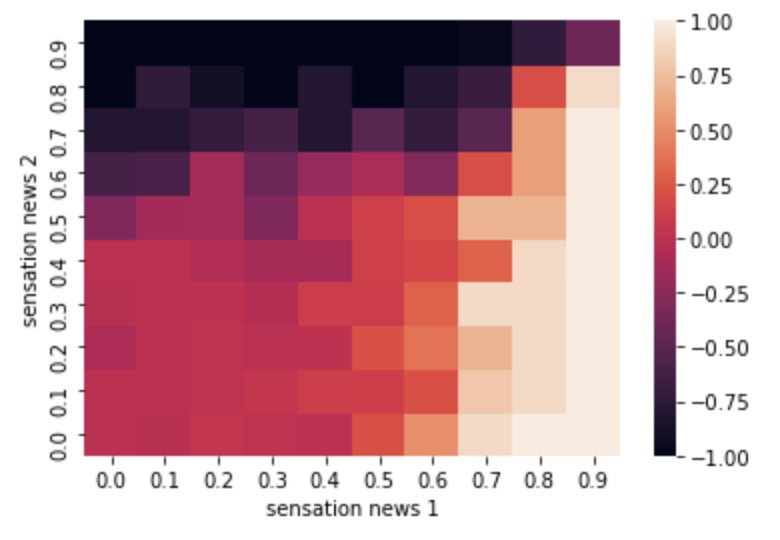
\includegraphics[width=.5\linewidth]{images/sens_vs_sens.png}
        \caption{Difference in fraction of nodes covered of two news with different sensations}
        \label{fig:sens_vs_sens}
    \end{figure}
\end{frame}

\begin{frame}{Choice of initial Set}
    News $N_1$ is started from the 5 most degree central nodes in both cases.
    \begin{figure}
      \centering
      \subfloat[$N_2$ started at 200 random nodes]{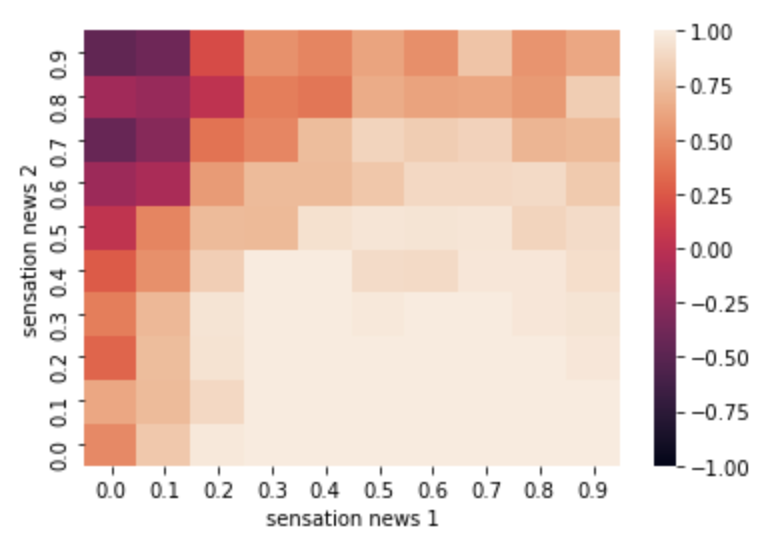
\includegraphics[height=4cm,width=4cm]{images/asize200.png}}\qquad
      \subfloat[$N_2$ started at 20 degree central nodes]{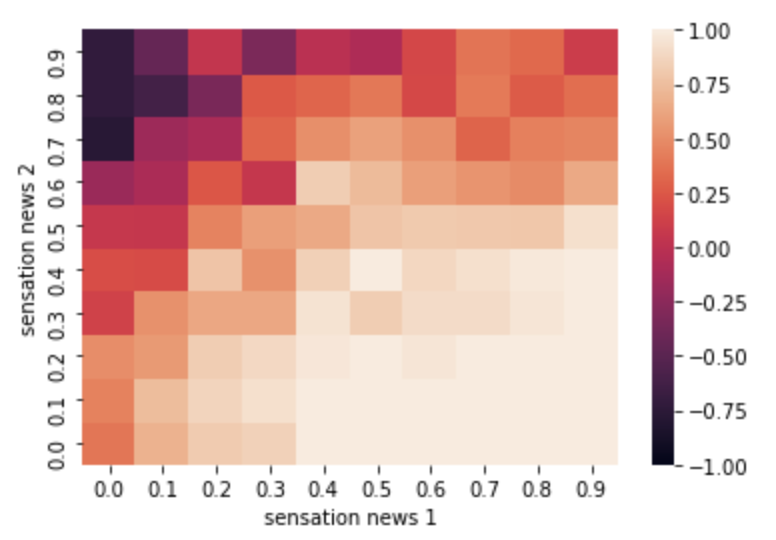
\includegraphics[height=4cm,width=4cm]{images/kset20.png}}
    \caption{Difference in fraction of nodes covered for different starting sets (1000 agents total)}
    \end{figure}
    20 well chosen nodes are already better than 200 randomly chosen nodes!
\end{frame}

\begin{frame}{Choice of initial Set}
    Another example:
    \begin{figure}
      \centering
      \subfloat[$N_2$ started at 500 random nodes]{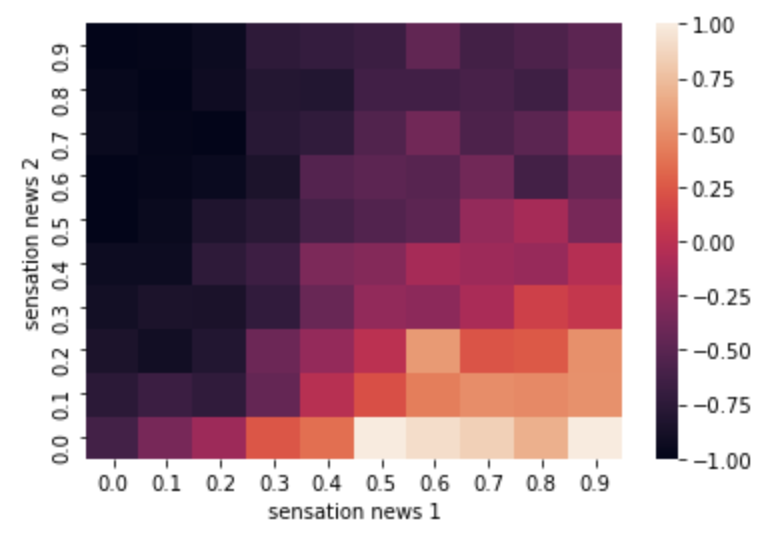
\includegraphics[height=4cm,width=4cm]{images/asize500.png}}\qquad
      \subfloat[$N_2$ started at 50 degree central nodes]{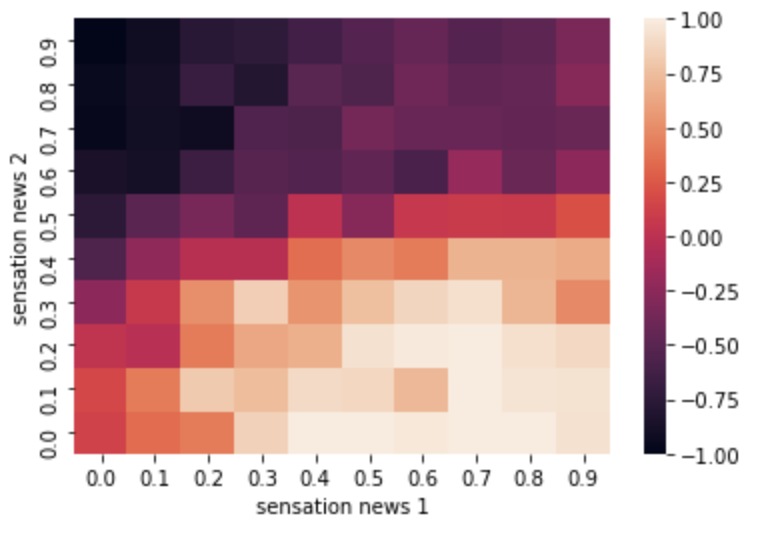
\includegraphics[height=4cm,width=4cm]{images/kset50.png}}
    \caption{Difference in fraction of nodes covered for different starting sets (1000 agents total)}
    \end{figure}
\end{frame}

\begin{frame}{Choice of initial Set: Greedy approximation}
    "Maximizing the Spread of Influence through a Social Network"\footnotemark, show
    \begin{enumerate}
        \item [1.] NP-hard problem
        \item [2.] A $(1-e)$-approximation is possible using a greedy algorithm
    \end{enumerate}
    Greedy algorithm in our network model:
    \begin{figure}
        \centering
        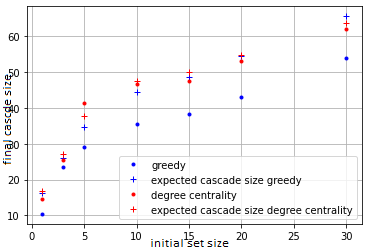
\includegraphics[width=.4\linewidth]{images/greedy.png}
        \caption{Actual and estimated cascade size of the same news in a 100 agent network with different starting sets}
    \end{figure}
    \footnotetext[1]{Kempe, David, Jon Kleinberg, and Éva Tardos. "Maximizing the spread of influence through a social network." Proceedings of the ninth ACM SIGKDD international conference on Knowledge discovery and data mining. 2003.}
\end{frame}

\begin{frame}{Choice of initial Set: Greedy approximation}
    Reasons why the greedy approximation performs worse:
    \begin{enumerate}
        \item [1.] Our greedy implementation is quite slow (Python) so the experiment was done with only 100 agents. There could be different result for larger networks
        \item[2.] Because we augmented our model with additional parameters, such as news sensation and agent independence, the greedy approximation might need to take them into consideration.
        \item[3.] Our model is directed where the standard threshold model is not.
    \end{enumerate}
\end{frame}

\begin{frame}{Choice of initial Set: Greedy approximation}
    Possible reasons why the greedy approximation performs worse in our model:
    \begin{enumerate}
        \item [1.] Our greedy implementation is quite slow (Python) so the experiment was done with only 100 agents. There could be different result for larger networks
        \item[2.] Because we augmented our model with additional parameters, such as news sensation and agent independence, the greedy approximation might need to take them into consideration.
        \item[3.] Our model uses a directed graph where the standard threshold model does not.
    \end{enumerate}
\end{frame}

\begin{frame}{Delay between News}
\begin{enumerate}
    \item [1.] At $t=0$ news 1 is launched by the most influential agent (highest degree).
    \item [2.] After some delay news 2 is launched as a "counter" at 5 influential agents.
\end{enumerate}
    \begin{figure}
    \centering
    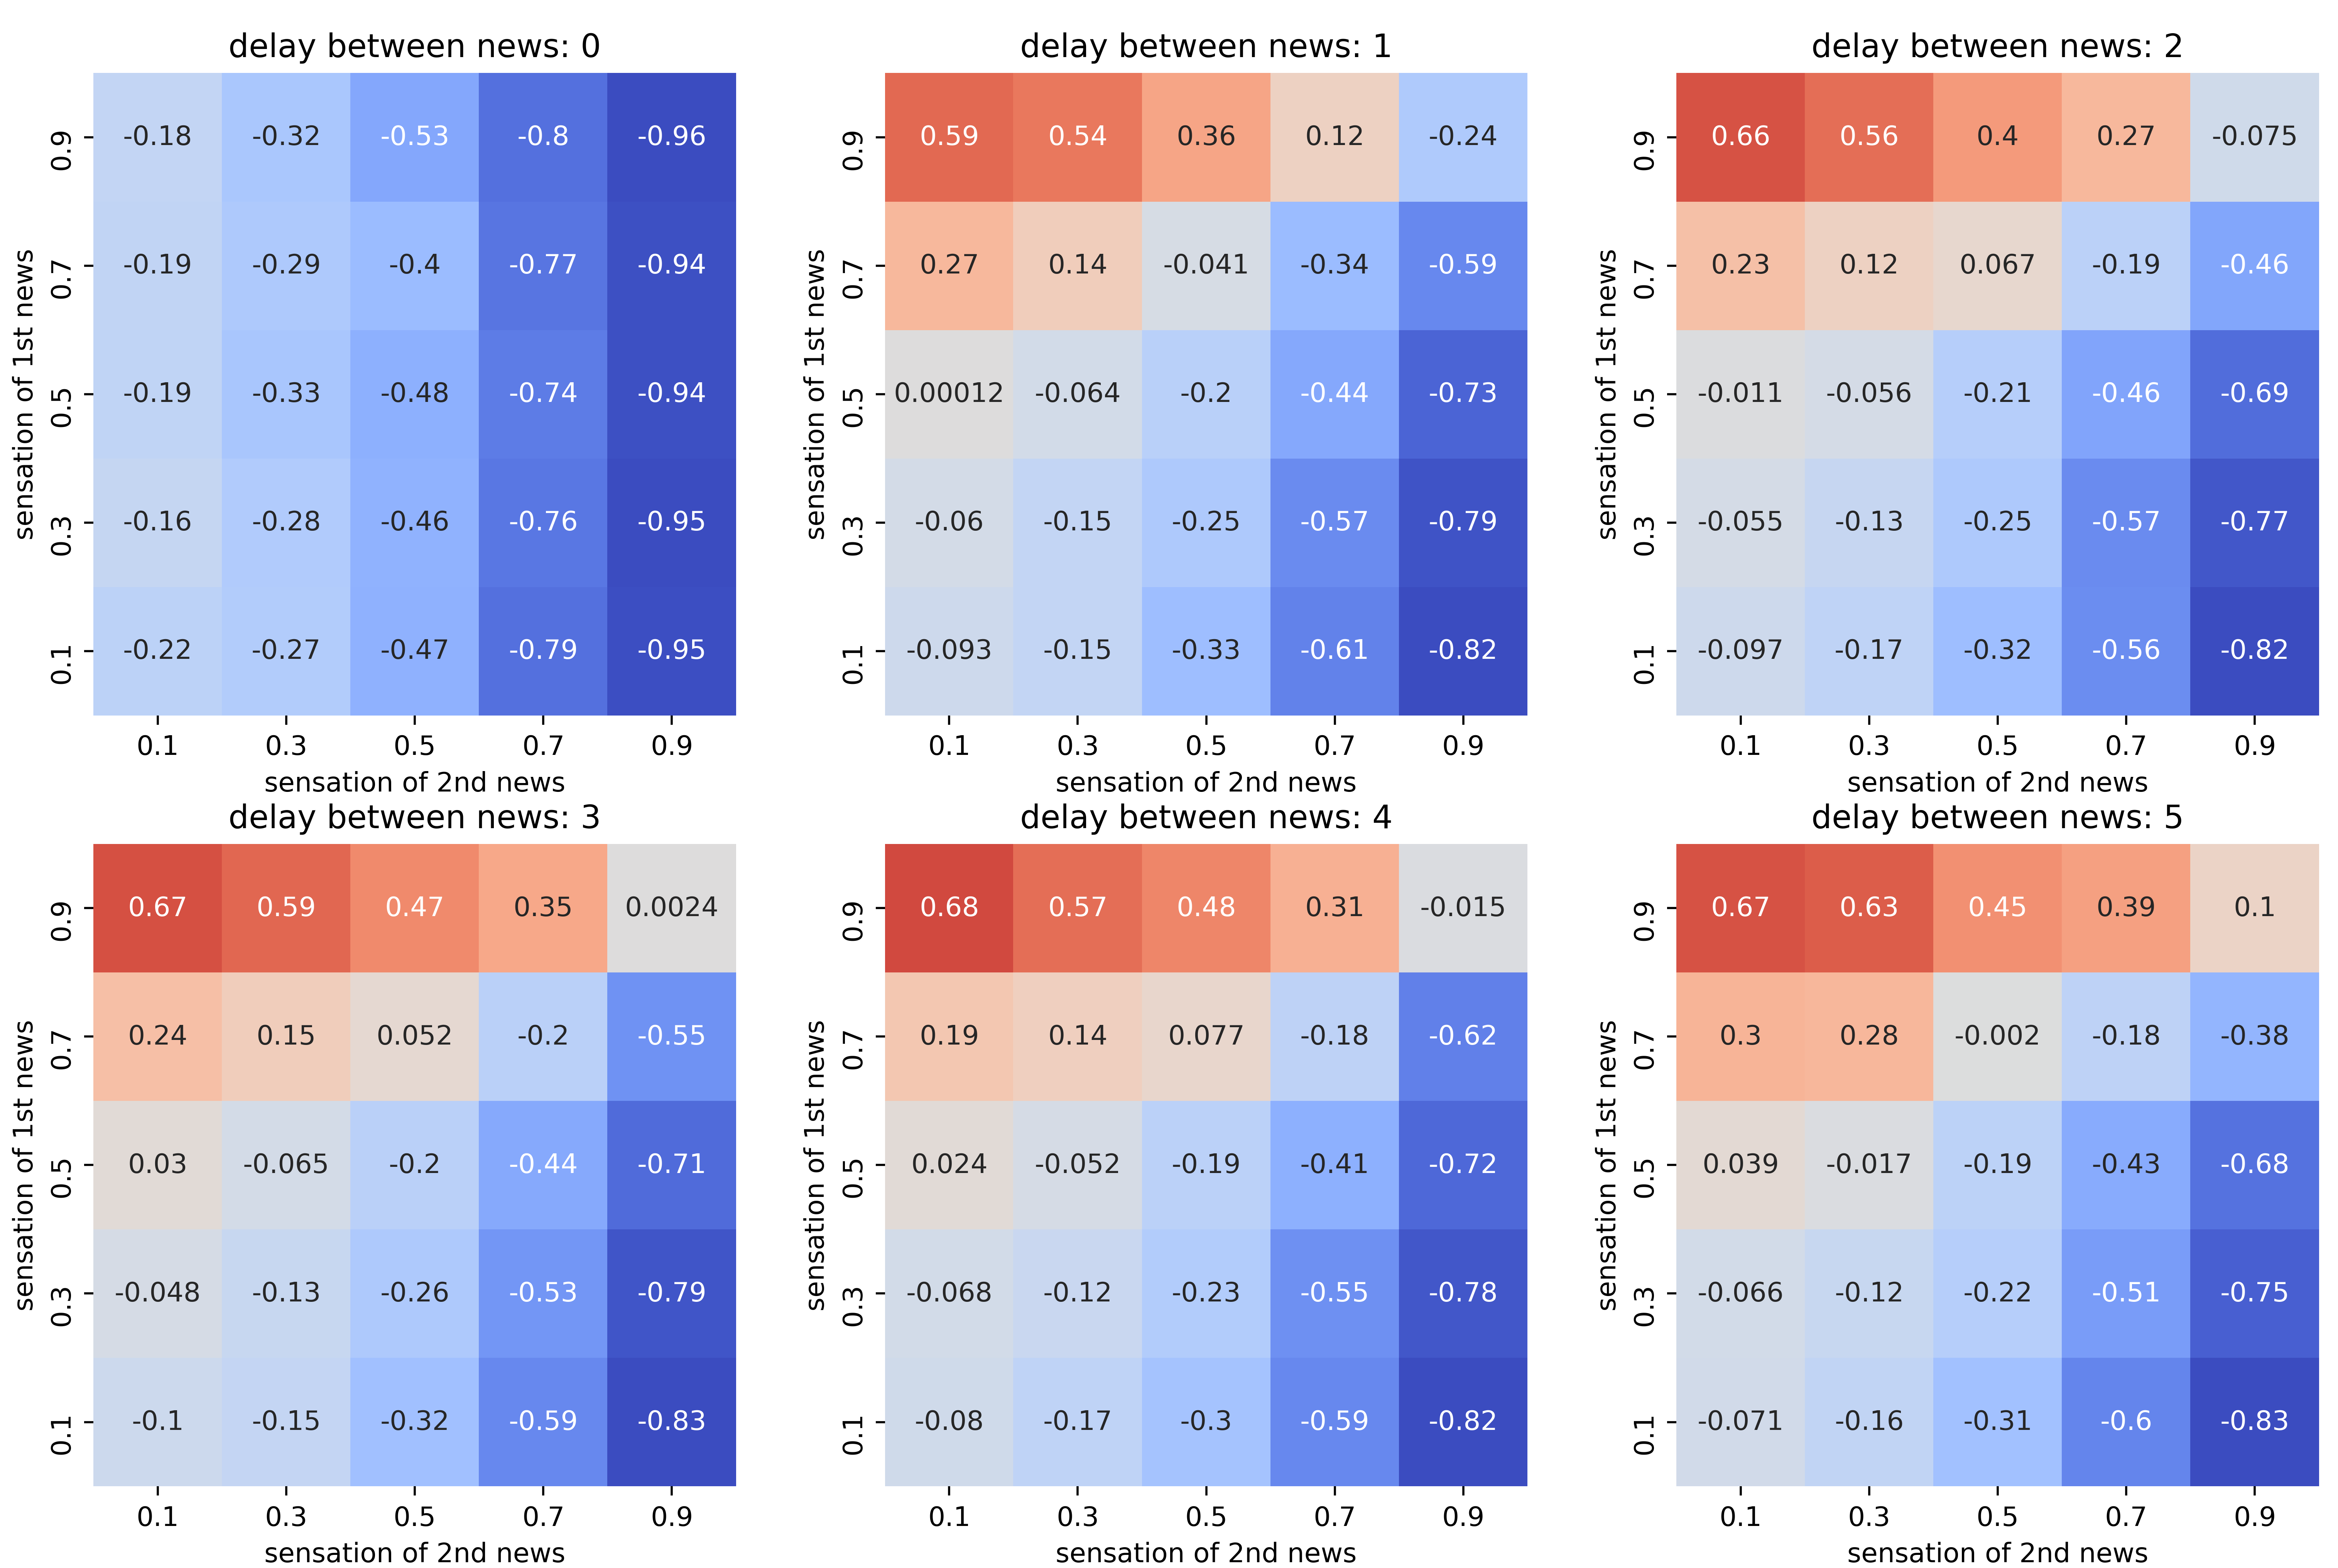
\includegraphics[width=.65\linewidth]{images/two_news_delays_no_decay_cut.png}
    \caption{Difference in fraction of nodes covered of two news with different delays}
    \end{figure}
\end{frame}

\begin{frame}{Delay between News}
    We find:
    \begin{enumerate}
        \item [-] The Delay has almost no effect except if it is 0.
        \item [-] If news 1 is given even a small advantage in time it will cover a lot of agents that news 2 does not manage to "flip".
    \end{enumerate}
\end{frame}

\section{Conclusion}

\begin{frame}{Limitations}
\begin{center}
    "All models are wrong, but some are useful" 
    - George Box
\end{center}
\end{frame}

\begin{frame}{Limitations}
Some limitations of our model are the following:
\begin{itemize}
\item<1-> Time is not properly modelled in the spreading dynamics (infection batches).
\item<2-> Scaling issues.
\end{itemize}
\end{frame}

\begin{frame}{Discussion}
Tell us what you think!
\end{frame}



\end{document}